\chapter{जीनोम स्थायित्व: DNA क्षति, मरम्मत और पुनर्संयोजन}\label{ch:b3:dna-repair}

समुद्र-तट पर बिताई एक दोपहर धूप में पड़ी हर त्वचा-कोशिका के DNA में
कोई लाख रासायनिक \omterm{def:b3:dna-repair:lesions}{विक्षतियाँ} डाल देती है: पराबैंगनी प्रकाश से जुड़कर
द्विलक बने पास-पास के थाइमीन, ऑक्सीकृत क्षार, कटी लड़ियाँ। बिना किसी
धूप के भी, कोशिका का गुनगुना पानी हर दिन लगभग दस हज़ार प्यूरीन अपनी
शर्कराओं से झाड़ देता है और सैकड़ों साइटोसीन यूरैसिल में बदल देता है।
फिर भी किसी मानव कोशिका की उत्परिवर्तन-दर प्रति विभाजन दस अरब क्षार
युग्मों में लगभग एक बदलाव है --- छह अरब के जीनोम में, प्रति विभाजन एक
नए उत्परिवर्तन से भी कम। कोई जीनोम जो क्षति भोगता है और जो क्षति रख
लेता है, उनके बीच की खाई मरम्मत भरती है: एक दर्जन एंज़ाइम-तंत्र जो
दोहरी कुंडली पर गश्त लगाते हैं, पहचानते हैं कि वहाँ क्या नहीं होना
चाहिए, उसे काटकर निकालते हैं और अक्षत लड़ी से फिर बनाते हैं, और जब
दोनों लड़ियाँ टूटी हों तो उन्हें फिर जोड़ते हैं या छूटा टुकड़ा किसी
सहोदरी से नकल कर लेते हैं। जिन बच्चों में इनमें से कोई एक तंत्र नहीं
है --- जो धूप के पहले स्पर्श से ही जल उठते हैं, या तीस के दशक में
बृहदांत्र-कर्कट पा जाते हैं --- वे दिखा देते हैं कि ये तंत्र किस मोल
के हैं। यह अध्याय क्षति के बारे में है, मरम्मत-पथों के बारे में, उस
पुनर्संयोजन तंत्र के बारे में जो सबसे बुरे विखंडनों की मरम्मत करता है
और जिसे अर्धसूत्री विभाजन उधार लेता है, और कोशिका के उस निर्णय के बारे
में कि मरम्मत विफल होने पर वह विभाजित होना छोड़ दे या मर जाए।

\section{DNA के साथ क्या-क्या गलत होता है}

\begin{definition}[DNA विक्षतियाँ]\label{def:b3:dna-repair:lesions}
\index{DNA विक्षति}\index{विप्यूरीनन}\index{विअमीनन}\index{पिरिमिडीन द्विलक}\index{द्विलड़ी विखंडन}\index{8-ऑक्सोग्वानीन}
\emph{विक्षति} DNA का ऐसा कोई भी रासायनिक परिवर्तन है जो अक्षत आधार-ढाँचे
पर सही ढंग से युग्मित चार सामान्य क्षारों से हटकर हो। स्वतःस्फूर्त
विक्षतियाँ पानी और ऑक्सीजन की रसायन से उठती हैं: \emph{विप्यूरीनन},
यानी किसी प्यूरीन और उसकी शर्करा के बीच के बंध का जल-अपघटन, जो कोई
अक्षारीय स्थल छोड़ जाता है (प्रति कोशिका प्रति दिन लगभग $10^{4}$);
\emph{विअमीनन}, जो साइटोसीन को यूरैसिल में, 5-मेथिलसाइटोसीन को थाइमीन
में और ऐडेनीन को हाइपोज़ैंथीन में बदल देता है (प्रति दिन कुछ सौ);
क्रियाशील ऑक्सीजन स्पीशीज़ से \emph{ऑक्सीकरण}, मुख्यतः
\emph{8-ऑक्सोग्वानीन} तक, जो ऐडेनीन से उतनी ही सहजता से युग्मित होता है
जितनी साइटोसीन से; और \emph{प्रतिकृति त्रुटियाँ}, यानी कोई गलत बैठा या
फिसला क्षार। परिवेशी विक्षतियों में हैं दो पास-पास के पिरिमिडीनों के
बीच पराबैंगनी प्रकाश से बना \emph{साइक्लोब्यूटेन पिरिमिडीन द्विलक} और
6-4 प्रकाशोत्पाद; क्षारकारी कारकों से बने क्षारकृत क्षार
(O$^{6}$-मेथिल-\linebreak[0]ग्वानीन थाइमीन से युग्मित होता है); ऐरोमैटिक
हाइड्रोकार्बनों और ऐफ़्लाटॉक्सिन से बने स्थूल योगज; सिसप्लैटिन और
नाइट्रोजन मस्टर्डों से बनी अंतर-लड़ी तिर्यक-कड़ियाँ; और आयनकारी विकिरण
से बने एकलड़ी तथा \emph{द्विलड़ी विखंडन}, प्रति कोशिका प्रति ग्रे लगभग
\num{1000} एकलड़ी और \numrange{30}{40} द्विलड़ी विखंडन।
\end{definition}

\begin{proposition}[निष्ठा की सीढ़ी]\label{prop:b3:dna-repair:fidelity}
\index{निष्ठा}\index{शुद्धि-पाठन}\index{असंगति मरम्मत}
प्रतिकृति प्रति क्षार युग्म लगभग $10^{-10}$ की अपनी त्रुटि-दर तीन
गुणात्मक चरणों में पाती है। ज्यामिति और हाइड्रोजन आबंधन के आधार पर
पॉलीमरेज़ का क्षार-चयन लगभग $10^{5}$ में एक बार चूकता है; पॉलीमरेज़ के
3$'\to$5$'$ एक्सोन्यूक्लिएज़ का \emph{शुद्धि-पाठन}, जो दीर्घन से पहले
किसी गलत युग्मित अंतिम क्षार को उच्छेदित कर देता है, उनमें से
\qty{99}{\%} हटा देता है; \emph{\omterm{prop:b3:dna-repair:fidelity}{असंगति मरम्मत}}, जो द्विशाख के पीछे नई
बनी लड़ी पर काम करती है, शेष का \qty{99.9}{\%} हटा देती है। गुणनफल
$10^{-5}\times 10^{-2}\times 10^{-3} = 10^{-10}$ ही प्रेक्षित दर है,
और दोनों संशोधन-चरणों में से किसी एक की भी खराबी उसे सौ या हज़ार गुना
बढ़ा देती है: ऐसी कोशिकाएँ \emph{उत्परिवर्तक} हैं।
\end{proposition}

\begin{example}[विक्षतियाँ बनाम उत्परिवर्तन]\label{ex:b3:dna-repair:numbers}
$6.4\times 10^{9}$ क्षार युग्मों वाली कोई मानव कोशिका जो दिन में एक बार
विभाजित होती है, प्रति दिन $10^{4}$--$10^{5}$ की कोटि की \omterm{def:b3:dna-repair:lesions}{विक्षतियाँ} और
प्रति विभाजन लगभग $6.4\times 10^{9}\times 10^{-10} \approx 0.6$ नए
उत्परिवर्तन जमा करती है: दस हज़ार \omterm{def:b3:dna-repair:lesions}{विक्षतियों} में से एक से भी कम स्थायी
बदलाव बनने तक बचती है। शेष की मरम्मत प्रतिकृति के उन्हें पढ़ने से पहले
हो जाती है, और चयन ने क्षति की दर नहीं, उत्परिवर्तन तक बच निकलने की दर
न्यूनतम की है। यही अंकगणित दिखाता है कि किसी अर्बुद में या किसी बड़ी
उम्र के पिता के शुक्राणु में उत्परिवर्तनों की संख्या विभाजन क्यों गिनती
है: कोई कोशिका जितने उत्परिवर्तन ढोती है वे, पहली कोटि में, उसके
विभाजनों की संख्या गुणा प्रति विभाजन त्रुटि हैं।
\end{example}

\section{एक क्षतिग्रस्त लड़ी की मरम्मत}

\begin{definition}[उच्छेदन मरम्मत]\label{def:b3:dna-repair:excision}
\index{क्षार-उच्छेदन मरम्मत}\index{न्यूक्लियोटाइड-उच्छेदन मरम्मत}\index{ग्लाइकोसिलेज़}\index{ज़ीरोडर्मा पिग्मेंटोसम}
अधिकांश \omterm{def:b3:dna-repair:lesions}{विक्षतियाँ} एक ही लड़ी पर पड़ती हैं और उनकी मरम्मत क्षतिग्रस्त
टुकड़ा काटकर दूसरी लड़ी की नकल करके होती है। \emph{क्षार-उच्छेदन मरम्मत}
(BER) छोटी, विरूपण न करने वाली \omterm{def:b3:dna-repair:lesions}{विक्षतियाँ} सँभालती है: किसी एक प्रकार के
गलत क्षार के लिए विशिष्ट कोई \emph{DNA ग्लाइकोसिलेज़}
(यूरैसिल-DNA ग्लाइकोसिलेज़, 8-ऑक्सोG ग्लाइकोसिलेज़, और कई दूसरी) क्षार
को कुंडली से बाहर पलट देती है और उसकी शर्करा से काट देती है; कोई AP
एंडोन्यूक्लिएज़ अक्षारीय स्थल पर आधार-ढाँचे में कटान लगाती है; कोई
पॉलीमरेज़ (Pol~$\beta$) शर्करा हटाकर एक न्यूक्लियोटाइड बैठा देती है;
कोई लाइगेज़ जोड़ देती है। \emph{न्यूक्लियोटाइड-उच्छेदन मरम्मत}
(NER) स्थूल, कुंडली को विरूपित करने वाली \omterm{def:b3:dna-repair:lesions}{विक्षतियाँ} --- \omterm{def:b3:dna-repair:lesions}{पिरिमिडीन
द्विलक}, रासायनिक योगज --- स्वयं \omterm{def:b3:dna-repair:lesions}{विक्षति} की रसायन पहचाने बिना सँभालती
है: विरूपण पकड़ा जाता है (जीनोम छानते XPC से, या अनुलेखन-युग्मित शाखा
में किसी रुकी RNA पॉलीमरेज़ से), TFIIH की हेलिकेज़ उपइकाइयाँ कुंडली
खोलती हैं, क्षति की पुष्टि होती है (XPA), दो एंडोन्यूक्लिएज़ (XPF, XPG)
क्षतिग्रस्त लड़ी को \numrange{24}{32} न्यूक्लियोटाइड की दूरी पर काटती
हैं, ऑलिगोन्यूक्लियोटाइड निकल जाता है, और पॉलीमरेज़ तथा लाइगेज़ अंतराल
भर देती हैं। सात XP प्रोटीनों में से किसी का भी ह्रास
\emph{ज़ीरोडर्मा पिग्मेंटोसम} पैदा करता है: धूप के प्रति अत्यधिक
संवेदनशीलता, झाइयाँ, और त्वचा-कर्कट की हज़ार गुना बढ़ी हुई दर।
\end{definition}

\begin{proof}[प्रमाण-सामग्री]
क्लीवर (1968) ने \omterm{def:b3:dna-repair:excision}{ज़ीरोडर्मा पिग्मेंटोसम} के रोगियों के त्वचा-तंतुकोरक
संवर्धित किए, उन्हें पराबैंगनी प्रकाश से विकिरित किया और S प्रावस्था
से बाहर रेडियोधर्मी थायमिडीन दिया। सामान्य कोशिकाओं ने अनेक छोटे
स्थलों पर चिह्न ग्रहण किया --- मरम्मत-चकत्तियों का ``अननुसूचित DNA
संश्लेषण'' --- जबकि रोगियों की कोशिकाओं ने लगभग कुछ नहीं लिया, और वे उन
मात्राओं पर मर गईं जिन पर सामान्य कोशिकाएँ बच जाती हैं: यह रोग
द्विलकों को उच्छेदित करने में विफलता है। दो रोगियों की कोशिकाओं को
संलयित करने पर संकर में मरम्मत प्रायः लौट आती थी, क्योंकि हर कोशिका वह
देती थी जो दूसरी में नहीं थी; इसी कसौटी से रोगी पूरक समूहों A से G में
छाँटे गए, पथ के हर जीन के लिए एक, जीनों के क्लोनित होने से वर्षों पहले।
\end{proof}

\begin{omfigure}
\begin{tikzpicture}[every node/.style={font=\scriptsize}, >=stealth]
  % BER column
  \node[font=\small\bfseries] at (2.0,3.2) {क्षार-उच्छेदन मरम्मत};
  \foreach \y/\txt in {2.6/{क्षतिग्रस्त क्षार (U, 8-ऑक्सोG)}, 1.5/{ग्लाइकोसिलेज़ क्षार हटाती है}, 0.4/{AP एंडोन्यूक्लिएज़ कटान लगाती है}, -0.7/{Pol $\beta$ एक न्यूक्लियोटाइड भरती है, लाइगेज़ जोड़ती है}} {
    \draw[very thick, omDef] (0.2,\y) -- (3.8,\y); \draw[very thick, omDef] (0.2,\y-0.25) -- (3.8,\y-0.25);
    \node[right, align=left] at (0.2,\y-0.6) {\txt};
  }
  \fill[omThm] (2.0,2.6) circle (0.1);
  \draw[omThm, thick] (1.9,1.5) -- (2.1,1.5);
  \draw[white, very thick] (1.9,0.4) -- (2.1,0.4);
  \fill[omMeth!80!black] (2.0,-0.7) circle (0.1);
  % NER column
  \node[font=\small\bfseries] at (8.0,3.2) {न्यूक्लियोटाइड-उच्छेदन मरम्मत};
  \foreach \y/\txt in {2.6/{स्थूल विक्षति कुंडली विरूपित करती है; XPC बँधता है}, 1.5/{TFIIH कुंडली खोलता है, XPA पुष्टि करता है}, 0.4/{XPF और XPG 24--32 nt की दूरी पर काटती हैं}, -0.7/{पॉलीमरेज़ अंतराल भरती है, लाइगेज़ जोड़ती है}} {
    \draw[very thick, omDef] (6.2,\y) -- (9.8,\y); \draw[very thick, omDef] (6.2,\y-0.25) -- (9.8,\y-0.25);
    \node[right, align=left] at (6.2,\y-0.6) {\txt};
  }
  \draw[omThm, very thick] (7.8,2.6) -- (8.2,2.6) -- (8.2,2.75) -- (7.8,2.75) -- cycle;
  \draw[omDef, very thick] (7.2,1.5) .. controls (7.6,1.85) and (8.4,1.85) .. (8.8,1.5); \draw[omThm, very thick] (7.85,1.72) -- (8.15,1.72);
  \draw[very thick, white] (7.0,0.4) -- (9.0,0.4); \draw[omThm, thick, ->] (7.0,0.7) -- (7.0,0.48); \draw[omThm, thick, ->] (9.0,0.7) -- (9.0,0.48);
  \draw[very thick, omMeth!80!black] (7.0,-0.7) -- (9.0,-0.7);
\end{tikzpicture}

{\small दो उच्छेदन-पथ। क्षार-उच्छेदन (बाएँ) किसी एक विशिष्ट गलत क्षार
को उसके लिए समर्पित \omterm{def:b3:dna-repair:excision}{ग्लाइकोसिलेज़} से पहचानता है और एक न्यूक्लियोटाइड
बदल देता है। न्यूक्लियोटाइड-उच्छेदन (दाएँ) उस विरूपण को पहचानता है जो
कोई भी स्थूल \omterm{def:b3:dna-repair:lesions}{विक्षति} करती है, लड़ी को दोनों ओर काटता है और कोई तीस
न्यूक्लियोटाइड का चकत्ता बदल देता है (हरा)।}
\end{omfigure}

\begin{definition}[असंगति मरम्मत]\label{def:b3:dna-repair:mmr}
\index{असंगति मरम्मत!लड़ी-विभेदन}\index{लिंच संलक्षण}\index{सूक्ष्म-उपग्रह अस्थिरता}
\emph{\omterm{prop:b3:dna-repair:fidelity}{असंगति मरम्मत}} (MMR) उन गलत युग्मों और छोटे
अंतर्वेशन--विलोपन फंदों को सुधारती है जो शुद्धि-पाठन से बच निकलते हैं।
MutS प्रोटीन (मनुष्यों में MSH2--MSH6) किसी असंगति के विरूपण को
पहचानता है और, MutL (MLH1--PMS2) के साथ, किसी एक्सोन्यूक्लिएज़ को
अनुज्ञा देता है कि वह नई संश्लेषित लड़ी को पास के किसी कटान से लेकर
असंगति के पार तक अपघटित कर दे; अंतराल पॉलीमरेज़ फिर भर देती है।
कठिनाई \emph{लड़ी-विभेदन} की है: किसी असंगति में दो क्षार होते हैं और
गलत केवल एक। \emph{Escherichia coli} में नई लड़ी इसलिए पहचानी जाती है
कि वह GATC स्थलों पर अभी मेथिलित नहीं हुई, जिन्हें Dam मेथिलेज़
संश्लेषण के कुछ मिनट बाद चिह्नित करती है; MutH अमेथिलित लड़ी में कटान
लगाती है। सुकेंद्रकियों में नई लड़ी ओकाज़ाकी खंडों के बीच के कटानों और
अग्रणी लड़ी के मुक्त 3$'$ सिरे से पहचानी जाती है। MMR का ह्रास
उत्परिवर्तन-दर सौ से हज़ार गुना बढ़ा देता है, और सबसे स्पष्ट रूप से
\emph{सूक्ष्म-उपग्रहों} पर --- किसी छोटी पुनरावृत्ति की ऐसी लड़ियाँ जहाँ
पॉलीमरेज़ फिसलती है --- जिनकी लंबाइयाँ कोशिका-दर-कोशिका बदलती हैं:
\emph{सूक्ष्म-उपग्रह अस्थिरता}। किसी एक MMR युग्मविकल्पी का वंशागत ह्रास
\emph{लिंच संलक्षण} है, जिसमें लगभग \qty{70}{\%} वाहकों को
बृहदांत्र-कर्कट होता है, प्रायः पचास से पहले।
\end{definition}

\begin{omfigure}
\begin{tikzpicture}[every node/.style={font=\scriptsize}, >=stealth]
  \draw[very thick, omDef] (0,1.2) -- (9,1.2); \node[left] at (-0.1,1.2) {साँचा-लड़ी};
  \draw[very thick, gray] (0,0.6) -- (9,0.6); \node[left] at (-0.1,0.6) {नई लड़ी};
  % methyl groups on template at GATC
  \foreach \x in {1.5,7.5} { \fill[omMeth!80!black] (\x,1.35) circle (0.1); \node[above] at (\x,1.45) {GATC पर CH$_3$}; }
  \foreach \x in {1.5,7.5} { \draw[omMeth!80!black] (\x,0.45) circle (0.1); }
  \node[below] at (7.5,0.32) {अभी मेथिलित नहीं};
  % mismatch
  \draw[omThm, very thick] (4.5,1.05) -- (4.5,0.75); \node[omThm, right] at (4.6,0.9) {असंगति};
  \draw[thick, fill=omExo!35] (4.5,1.9) ellipse (1.0 and 0.3); \node at (4.5,1.9) {MutS/MutL};
  \draw[->, thick] (4.5,1.65) -- (4.5,1.3);
  % MutH nick on new strand at unmethylated GATC
  \draw[omThm, thick, ->] (1.5,-0.55) -- (1.5,0.42); \node[omThm, below] at (1.5,-0.55) {MutH अमेथिलित लड़ी में कटान लगाती है};
  % excision arrow
  \draw[->, very thick, omProp] (1.7,-0.1) -- (5.0,-0.1); \node[omProp, below] at (3.95,-0.15) {एक्सोन्यूक्लिएज़ असंगति के पार तक अपघटित करती है};
  \node[right] at (5.4,-0.8) {फिर Pol III अंतराल भरती है, लाइगेज़ जोड़ती है};
\end{tikzpicture}

{\small जीवाणुओं की \omterm{prop:b3:dna-repair:fidelity}{असंगति मरम्मत} में लड़ी-विभेदन। साँचा-लड़ी अपने GATC
स्थलों पर मेथिल समूह ढोती है; नई लड़ी अभी नहीं ढोती, और MutH वहीं उसमें
कटान लगाती है। इसलिए गलत क्षार सदा नई लड़ी से ही हटाया जाता है।}
\end{omfigure}

\begin{method}[किसी मरम्मत-रोग को जीनों में छाँटना]\label{met:b3:dna-repair:complementation}
\index{पूरकता परीक्षण}
किसी अप्रभावी लक्षण-प्ररूप में कितने जीन शामिल हैं, यह किसी भी जीन के
ज्ञात होने से पहले जानने के लिए: (1) असंबंधित रोगियों से कोशिका-वंश
लीजिए, जिनमें से हर एक पथ के किसी न किसी जीन में उत्परिवर्ती हो;
(2) वंशों के युग्मों को संलयित करके संकर कोशिकाएँ बनाइए; (3) संकर में
प्रकार्य की जाँच कीजिए (यहाँ, पराबैंगनी प्रकाश के बाद अननुसूचित DNA
संश्लेषण); (4) यदि संकर में मरम्मत हो जाए तो दोनों रोगियों के
उत्परिवर्तन \emph{भिन्न} जीनों में हैं (हर एक दूसरे का छूटा प्रोटीन
देता है: वे \emph{पूरक} हैं); न हो तो एक ही जीन में; (5) रोगियों को
पूरक समूहों में बाँटिए --- प्रति जीन एक। समूहों की गिनती जीनों की
संख्या की निचली सीमा है।
\end{method}

\section{किसी टूटे गुणसूत्र की मरम्मत}

\begin{definition}[द्विलड़ी विखंडन की मरम्मत]\label{def:b3:dna-repair:dsb}
\index{असमजात सिरा-संयोजन}\index{समजात पुनर्संयोजन}\index{Rad51}\index{हॉलिडे संधि}\index{BRCA}
कोई \emph{\omterm{def:b3:dna-repair:lesions}{द्विलड़ी विखंडन}} गुणसूत्र को काट देता है और नकल करने के लिए
कोई अक्षत लड़ी नहीं छोड़ता। दो पथ उसकी मरम्मत करते हैं। \emph{असमजात
सिरा-संयोजन} (NHEJ): Ku70--Ku80 वलय हर सिरे से बँधता है, काइनेज़
DNA-PKcs को बुलाता है, न्यूक्लिएज़ अधिलंब छाँटती हैं, और लाइगेज़ IV
सिरे जोड़ देती है; यह चक्र की किसी भी अवस्था में और मिनटों में काम करता
है, पर संधि पर कुछ न्यूक्लियोटाइड खो या जोड़ देता है और गलत सिरे भी
जोड़ सकता है। \emph{समजात पुनर्संयोजन} (HR): MRN संकुल और
न्यूक्लिएज़ 5$'$ लड़ियों का अपच्छेदन करके लंबी 3$'$ एकलड़ी पूँछें छोड़ते
हैं, जिन्हें RPA और फिर, BRCA2 की सहायता से, पुनर्संयोजक \emph{Rad51}
ढक लेता है; Rad51 तंतु किसी समजात द्विकुंडली की खोज करता है --- S और G2
में सहोदरी क्रोमैटिड --- उसमें प्रवेश करता है, और प्रवेश करता 3$'$ सिरा
अक्षत प्रति पर संश्लेषण आरंभ कर देता है। संयुक्त अणु या तो थोड़े
संश्लेषण के बाद घोल दिए जाते हैं (अधिकांश समसूत्री मरम्मत, पार्श्व DNA
का कोई विनिमय नहीं) या दो चतुर्भुजी \emph{हॉलिडे संधियों} में परिपक्व
होते हैं, जिनका एंडोन्यूक्लिएज़ों द्वारा विभेदन या तो कोई जीन-विनिमय
देता है या कोई अ-विनिमय उत्पाद। HR यथार्थ है क्योंकि वह किसी सहोदरी की
नकल करता है, पर वह तभी उपलब्ध है जब कोई सहोदरी हो।
\end{definition}

\begin{omfigure}
\begin{tikzpicture}[every node/.style={font=\scriptsize}, >=stealth]
  % break
  \draw[very thick, omDef] (0,3.2) -- (2.3,3.2); \draw[very thick, omDef] (2.7,3.2) -- (5,3.2);
  \draw[very thick, omDef] (0,3.0) -- (2.3,3.0); \draw[very thick, omDef] (2.7,3.0) -- (5,3.0);
  \node[above] at (2.5,3.3) {द्विलड़ी विखंडन};
  % NHEJ left
  \draw[->, thick] (1.2,2.8) -- (-0.5,2.0); \node[left, align=right] at (-0.6,2.4) {कोई भी प्रावस्था,\\मिनट};
  \node[font=\small\bfseries] at (-1.6,1.55) {NHEJ};
  \draw[thick, fill=omExo!35] (-2.6,0.9) ellipse (0.3 and 0.2); \draw[thick, fill=omExo!35] (-0.8,0.9) ellipse (0.3 and 0.2);
  \draw[very thick, omDef] (-3.4,0.9) -- (-2.9,0.9); \draw[very thick, omDef] (-0.5,0.9) -- (0.0,0.9);
  \node[below] at (-1.7,0.7) {Ku दोनों सिरों से बँधता है, छँटाई};
  \draw[->, thick] (-1.7,0.3) -- (-1.7,-0.1);
  \draw[very thick, omDef] (-3.4,-0.4) -- (0.0,-0.4); \draw[omThm, very thick] (-1.85,-0.4) -- (-1.55,-0.4);
  \node[below, align=center] at (-1.7,-0.55) {लाइगेज़ IV जोड़ती है:\\कुछ न्यूक्लियोटाइड खोए या जुड़े};
  % HR right
  \draw[->, thick] (3.8,2.8) -- (5.5,2.0); \node[right, align=left] at (5.6,2.4) {S/G2, कोई सहोदरी\\उपस्थित; घंटे};
  \node[font=\small\bfseries] at (6.8,1.55) {HR};
  % resected ends
  \draw[very thick, omDef] (4.6,0.9) -- (6.2,0.9); \draw[very thick, omDef] (7.4,0.9) -- (9.0,0.9);
  \draw[very thick, omDef] (4.6,0.7) -- (5.6,0.7); \draw[very thick, omDef] (8.0,0.7) -- (9.0,0.7);
  \foreach \x in {5.7,5.9,6.1} \fill[omProp] (\x,0.9) circle (0.07);
  \node[below] at (6.8,0.55) {5$'$ अपच्छेदन; Rad51 3$'$ पूँछें ढक लेता है};
  \draw[->, thick] (6.8,0.15) -- (6.8,-0.25);
  % strand invasion of sister
  \draw[very thick, omMeth!70!black] (4.6,-0.9) -- (9.0,-0.9); \draw[very thick, omMeth!70!black] (4.6,-1.1) -- (9.0,-1.1);
  \draw[very thick, omDef] (4.6,-0.5) -- (5.8,-0.5) .. controls (6.2,-0.5) and (6.3,-0.9) .. (6.6,-0.9) -- (7.6,-0.9);
  \draw[->, omDef, thick] (7.6,-0.9) -- (8.1,-0.9);
  \node[below, align=center] at (6.8,-1.2) {सहोदरी (हरी) में प्रवेश, अक्षत प्रति पर संश्लेषण,\\फिर विघटन (कोई जीन-विनिमय नहीं) या हॉलिडे संधियाँ};
\end{tikzpicture}

{\small किसी \omterm{def:b3:dna-repair:lesions}{द्विलड़ी विखंडन} की दो नियतियाँ। बाएँ: सिरा-संयोजन, तेज़ और
सदा उपलब्ध, संधि पर एक छोटे बदलाव की कीमत पर। दाएँ: \omterm{def:b3:dna-repair:dsb}{समजात पुनर्संयोजन},
जो सिरों का अपच्छेदन करता है, \omterm{def:b3:dna-repair:dsb}{Rad51} तंतु से सहोदरी क्रोमैटिड में प्रवेश
करता है और जो खोया था उसकी नकल कर लेता है।}
\end{omfigure}

\begin{theorem}[क्षति-भार, मरम्मत-दर और द्विशाख]\label{thm:b3:dna-repair:load}
\index{अवशिष्ट क्षति}\index{प्रतिस्पर्धी पथ}
मान लीजिए किसी एक प्रकार की \omterm{def:b3:dna-repair:lesions}{विक्षतियाँ} प्रति कोशिका प्रति घंटा अचर दर
$D$ से उठती हैं और दर-नियतांक $k$ वाली प्रथम-कोटि मरम्मत से हटती हैं
(अर्ध-आयु $t_{1/2} = \ln 2/k$)। \omterm{def:b3:dna-repair:lesions}{विक्षतियों} की संख्या $L(t)$
$\mathrm{d}L/\mathrm{d}t = D - kL$ का पालन करती है, इसलिए स्थायी अवस्था पर
\[
L^{*} = \frac{D}{k},
\]
और $N$ \omterm{def:b3:dna-repair:lesions}{विक्षतियों} का कोई स्फुरण, जो $t = 0$ पर दिया गया हो,
$N e^{-kT}$ \omterm{def:b3:dna-repair:lesions}{विक्षतियाँ} छोड़ता है जब कोई प्रतिकृति द्विशाख समय $T$ पर
पहुँचता है। यदि दो
पथ दर-नियतांक $k_{1}$ और $k_{2}$ के साथ एक ही \omterm{def:b3:dna-repair:lesions}{विक्षति} के लिए
प्रतिस्पर्धा करें, तो हर \omterm{def:b3:dna-repair:lesions}{विक्षति} की मरम्मत पहला पथ प्रायिकता
$k_{1}/(k_{1} +
k_{2})$ से करता है और कुल अर्ध-आयु $\ln 2/(k_{1} + k_{2})$ होती है।
द्विशाख तक पहुँचने वाली \omterm{def:b3:dna-repair:lesions}{विक्षतियों} की संख्या माध्य
$N e^{-kT}$ के साथ पॉइसों-वितरित है, इसलिए एक भी न पहुँचने की प्रायिकता $\exp(-N e^{-kT})$ है।
\end{theorem}
\begin{proof}
स्थायी अवस्था वहीं है जहाँ $D = kL$ हो। स्फुरण के लिए $D = 0$ है और
समीकरण का समाकलन $L = N e^{-kt}$ देता है। दो पथ होने पर ह्रास की
दर $(k_{1} + k_{2})L$ है; किसी भी छोटे अंतराल में कोई दी हुई \omterm{def:b3:dna-repair:lesions}{विक्षति}
पथ~1 से प्रायिकता $k_{1}\,\mathrm{d}t$ और पथ~2 से
$k_{2}\,\mathrm{d}t$ के साथ हटती है, इसलिए यह सप्रतिबंध प्रायिकता कि
उसका हटना, जब हो, पथ~1 से हो, $k_{1}/(k_{1} +
k_{2})$ है। स्वतंत्र \omterm{def:b3:dna-repair:lesions}{विक्षतियाँ}, जिनमें से हर एक प्रायिकता $e^{-kT}$ से
बचती है, कोई द्विपद गणना देती हैं, जो अनेक \omterm{def:b3:dna-repair:lesions}{विक्षतियों} और कम उत्तरजीविता
की सीमा में पॉइसों है, और शून्य की पॉइसों प्रायिकता $e^{-\text{माध्य}}$ है।
\end{proof}

\begin{example}[ज़ीरोडर्मा द्विशाख का रोग क्यों है]\label{ex:b3:dna-repair:xp}
धूप की एक मात्रा किसी शल्कीकोशिका में $N = 10^{5}$ \omterm{def:b3:dna-repair:lesions}{पिरिमिडीन द्विलक}
छोड़ जाती है। \qty{2}{h} के न्यूक्लियोटाइड-उच्छेदन अर्ध-आयु ($k =
\qty{0.35}{h^{-1}}$) और \qty{8}{h} बाद पहुँचते द्विशाख पर, $N e^{-kT} =
10^{5}\times e^{-2.8} \approx 6000$ द्विलक अब भी नकल होने को वहीं हैं;
किसी XP कोशिका की लगभग अनुपस्थित मरम्मत ($k \approx
\qty{0.01}{h^{-1}}$) पर \num{92000} हैं। द्विशाख से मिलता हर द्विलक
\omterm{def:b3:dna-repair:tls}{विक्षति-पार संश्लेषण} (नीचे) से लाँघा जाता है, जो त्रुटि-प्रवण है:
रोगी का प्रति विभाजन उत्परिवर्तन-भार सामान्य से पंद्रह गुना है, और
त्वचा-कर्कट बचपन में ही आ जाते हैं। जो उपचार काम करता है वह $N$ को छोटा
रखना है --- पराबैंगनी प्रकाश से पूर्ण परिहार।
\end{example}

\begin{omfigure}
\begin{tikzpicture}
\begin{axis}[
  width=0.7\linewidth, height=5.6cm,
  axis x line=bottom, axis y line=left,
  xmin=0, xmax=12, ymin=100, ymax=200000, ymode=log,
  xlabel={संपर्क के बाद के घंटे}, ylabel={प्रति कोशिका द्विलक},
  xlabel style={font=\small, at={(axis description cs:0.5,-0.12)}, anchor=north},
  ylabel style={font=\small},
  tick label style={font=\small}, xtick={0,2,4,6,8,10,12},
  clip=false,
]
\addplot[very thick, omDef, domain=0:12, samples=40] {100000*exp(-0.35*x)};
\addplot[very thick, omThm, domain=0:12, samples=40] {100000*exp(-0.01*x)};
\addplot[dashed, gray] coordinates {(8,100) (8,200000)};
\node[font=\scriptsize, anchor=south east, gray] at (axis cs:8,110) {द्विशाख पहुँचता है};
\node[font=\scriptsize, omDef, anchor=north east] at (axis cs:11.5,18000) {सामान्य, $t_{1/2} = \qty{2}{h}$};
\node[font=\scriptsize, omThm, anchor=south west] at (axis cs:2,105000) {ज़ीरोडर्मा पिग्मेंटोसम};
\fill[omDef] (axis cs:8,6070) circle (2pt); \node[font=\scriptsize, omDef, anchor=west] at (axis cs:8.3,6070) {\num{6000}};
\fill[omThm] (axis cs:8,92300) circle (2pt); \node[font=\scriptsize, omThm, anchor=north west] at (axis cs:8.3,80000) {\num{92000}};
\end{axis}
\end{tikzpicture}

{\small $10^{5}$ के एक स्फुरण के बाद बचे द्विलक, लघुगणकीय मापनी पर,
किसी सामान्य कोशिका और किसी न्यूक्लियोटाइड-उच्छेदन-अपर्याप्त कोशिका के
लिए। \qty{8}{h} पर द्विशाख रोगी की कोशिका में पंद्रह गुना अधिक
\omterm{def:b3:dna-repair:lesions}{विक्षतियों} से मिलता है।}
\end{omfigure}

\begin{proof}[प्रमाण-सामग्री]
हॉलिडे (1964) ने कवक-आनुवंशिकी की एक पहेली समझाने के लिए चतुर्भुजी
संधि प्रस्तावित की: किसी संकरण में बीजाणुओं का कोई चतुष्क कभी-कभी
किसी चिह्नक का $3{:}1$ पृथक्करण दिखाता था, मेंडेली $2{:}2$ के बजाय, और
सदा उन्हीं चिह्नकों के लिए जो किसी जीन-विनिमय के पास हों। उनका प्रतिरूप
--- दो समजात द्विकुंडलियों के बीच एकल लड़ियों का विनिमय, जिससे ऐसा
विषमयुग्मक बनता है जिसे \omterm{prop:b3:dna-repair:fidelity}{असंगति मरम्मत} फिर एक या दूसरी दिशा में ``सुधार''
देती है (\emph{जीन-परिवर्तन}) --- दोनों की व्याख्या करता था: विचित्र
अनुपातों की भी और जीन-विनिमय से उनके संबंध की भी। संधि स्वयं बाद में
पुनर्संयोजित हो रहे प्लाज़्मिडों में इलेक्ट्रॉन सूक्ष्मदर्शी से और उससे
बँधे विभेदक RuvC की संरचना में देखी गई।
\end{proof}

\section{सहिष्णुता, चेतावनी और रुकने का निर्णय}

\begin{definition}[विक्षति-पार संश्लेषण]\label{def:b3:dna-repair:tls}
\index{विक्षति-पार संश्लेषण}\index{पॉलीमरेज़ ईटा}
जब कोई द्विशाख ऐसी \omterm{def:b3:dna-repair:lesions}{विक्षति} से मिलता है जिसकी मरम्मत नहीं हुई, तो
प्रतिकृतिकारी पॉलीमरेज़ रुक जाती है। \emph{विक्षति-पार संश्लेषण} (TLS)
कोई ऐसी विशिष्ट पॉलीमरेज़ बुलाता है जिसका सक्रिय स्थल अधिक चौड़ा है और
जिसमें शुद्धि-पाठन नहीं --- \omterm{def:b3:dna-repair:lesions}{पिरिमिडीन द्विलकों} के लिए Pol~$\eta$, दूसरी
\omterm{def:b3:dna-repair:lesions}{विक्षतियों} के लिए Pol~$\iota$, $\kappa$, $\zeta$ और Rev1 --- जो \omterm{def:b3:dna-repair:lesions}{विक्षति}
के सामने कुछ न्यूक्लियोटाइड बैठाकर हट जाती है। Pol~$\eta$ किसी थाइमीन
द्विलक के सामने दो ऐडेनीन रखती है, जो प्रायः सही होता है; दूसरी अक्सर
गलत होती हैं। TLS यथार्थता देकर द्विशाख की उत्तरजीविता खरीदता है, और
पराबैंगनी-प्रेरित अधिकांश उत्परिवर्तनों का स्रोत है। \omterm{def:b3:dna-repair:excision}{ज़ीरोडर्मा
पिग्मेंटोसम} का विचरणी रूप (XP-V) अक्षत उच्छेदन मरम्मत रखता है और
Pol~$\eta$ से वंचित है: जो द्विलक उच्छेदन से बच जाते हैं उन्हें अधिक
त्रुटि-प्रवण पॉलीमरेज़ लाँघती हैं, और कर्कट पीछे-पीछे आ जाते हैं।
\end{definition}

\begin{proposition}[जीवाणुओं की SOS अनुक्रिया]\label{prop:b3:dna-repair:sos}
\index{SOS अनुक्रिया}\index{RecA}\index{LexA}
\emph{E.~coli} में पुनर्संयोजक RecA, जो रुके द्विशाखों और अपच्छेदित
विखंडनों पर जमा एकलड़ी DNA से बँधता है, ऐसा सह-प्रोटिएज़ बन जाता है जो
दमनकारी LexA को स्वयं को काटने के लिए प्रेरित करता है। LexA कोई चालीस
जीनों का दमन करता है; जैसे-जैसे वह गिरता है, वे अपने प्रचालकों की
आसक्ति के क्रम में चालू होते हैं: पहले उच्छेदन-मरम्मत जीन \emph{uvrA}
और \emph{uvrB}, फिर स्वयं \emph{recA} और कोशिका-विभाजन का निरोधक
\emph{sulA} (कोशिकाएँ विभाजित होना बंद कर देती हैं और तंतुओं में बढ़ती
हैं), और अंत में त्रुटि-प्रवण पॉलीमरेज़ Pol~IV तथा Pol~V, जो
उत्परिवर्तनों की कीमत पर \omterm{def:b3:dna-repair:lesions}{विक्षतियाँ} लाँघती हैं। यह श्रेणीबद्ध अनुक्रिया
पहले यथार्थ मरम्मत आज़माती है और उत्परिवर्तनकारी सहिष्णुता तभी, जब
क्षति बनी रहे; जो उत्परिवर्तन वह प्रेरित करती है वे वह कच्चा माल हैं
जिस पर उपचार के दौरान प्रतिजैविक प्रतिरोध विकसित होता है।
\end{proposition}

\begin{omfigure}
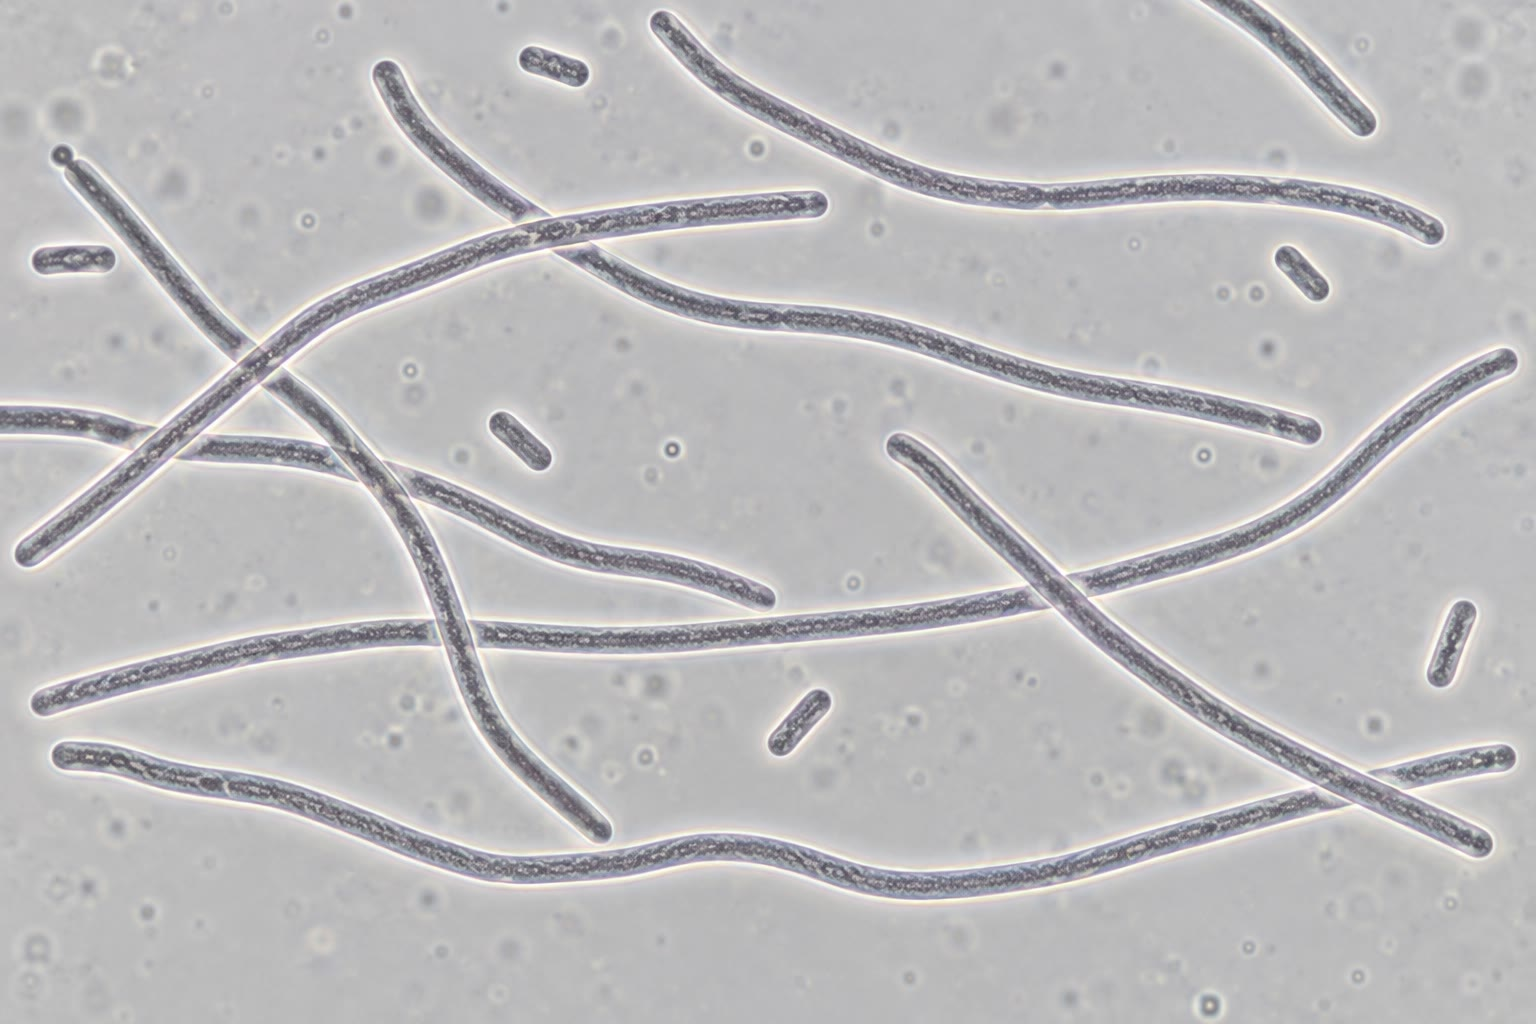
\includegraphics[width=0.46\linewidth]{images/book5/ai/b5-03-sos-filaments.jpg}\hspace{0.04\linewidth}
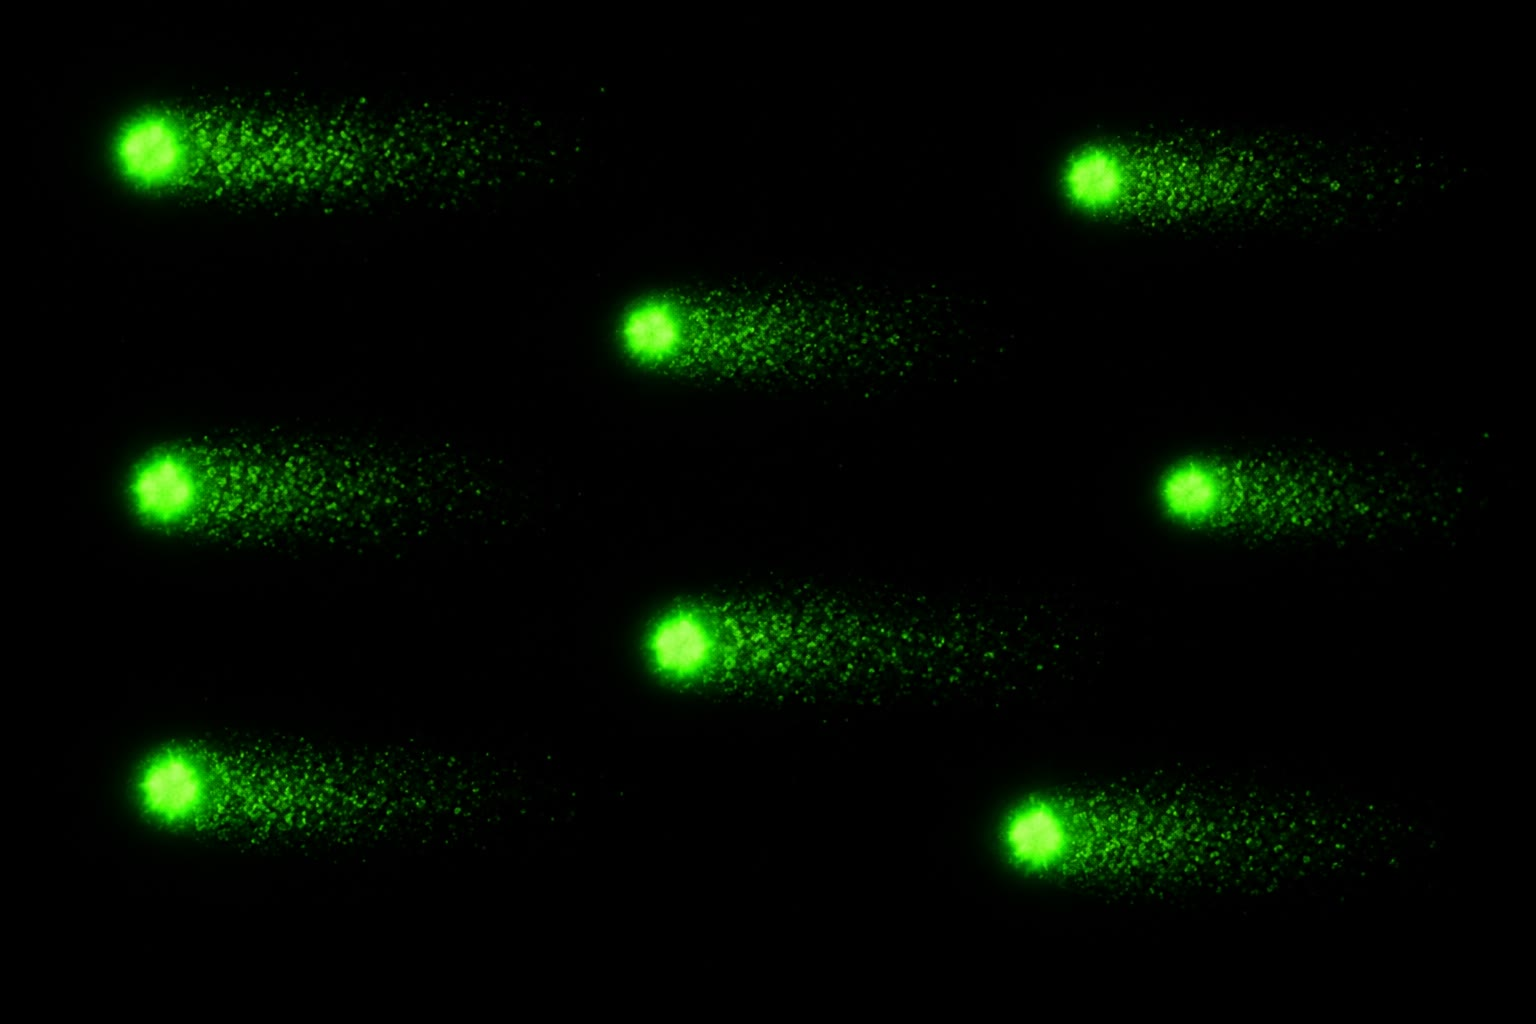
\includegraphics[width=0.46\linewidth]{images/book5/ai/b5-03-comet-assay.jpg}

{\small बाएँ: पराबैंगनी विकिरण के बाद \emph{E.~coli}, जो लंबे तंतुओं
में बढ़ गए हैं क्योंकि \omterm{prop:b3:dna-repair:sos}{SOS अनुक्रिया} ने DNA की मरम्मत होने तक
कोशिका-विभाजन रोक दिया है। दाएँ: कोई धूमकेतु परीक्षण --- अकेली
कोशिकाएँ किसी जेल में जड़ी और वैद्युत-कणसंचालित; खंडित DNA केंद्रक से
बहकर ऐसी पूँछ में निकल आता है जिसकी लंबाई विखंडनों की संख्या मापती है।}
\end{omfigure}

\begin{definition}[DNA क्षति अनुक्रिया]\label{def:b3:dna-repair:ddr}
\index{DNA क्षति अनुक्रिया}\index{ATM}\index{जाँच-बिंदु}\index{p53}\index{गामा-H2AX}
सुकेंद्रकी क्षति का संकेत दो काइनेज़ों से देते हैं: \emph{ATM}, जिसे MRN
संकुल \omterm{def:b3:dna-repair:lesions}{द्विलड़ी विखंडनों} तक बुलाता है, और \emph{ATR}, जिसे रुके द्विशाखों
का एकलड़ी DNA बुलाता है। वे सैकड़ों लक्ष्यों का फ़ॉस्फ़ोरिलन करते हैं।
मिनटों के भीतर हर विखंडन के चारों ओर मेगाक्षारों भर \omterm{def:b3:chromatin-epigenetics:nucleosome}{हिस्टोन} H2AX
फ़ॉस्फ़ोरिलित हो जाता है (\emph{$\gamma$-H2AX}) और ऐसा केंद्र बनता है
जो मरम्मत-प्रोटीनों को बुलाता है और सूक्ष्मदर्शी के नीचे गिना जा सकता
है, प्रति विखंडन एक केंद्र। काइनेज़ Chk1 और Chk2 कोशिका-चक्र रोक देती
हैं --- \cref{ch:b3:cell-cycle-apoptosis} के \emph{जाँच-बिंदु} --- उन
फ़ॉस्फ़ेटेज़ों को निष्क्रिय करके जो S या M में प्रवेश चलातीं; और
अनुलेखन-कारक \emph{p53}, जो फ़ॉस्फ़ोरिलन से स्थिर होता है, चक्रिन-निर्भर
काइनेज़ का निरोधक p21 (G1 में एक टिकाऊ विराम), मरम्मत-जीन, और यदि क्षति
भारी हो या बनी रहे तो वे मृत्युक जीन प्रेरित करता है जो कोशिका को मार
देते हैं। यह अनुक्रिया मरम्मत के लिए समय खरीदती है, और जब मरम्मत विफल
हो तो कोशिका को टूटे जीनोम के साथ विभाजित होने देने के बजाय हटा देती है।
\end{definition}

\begin{omfigure}
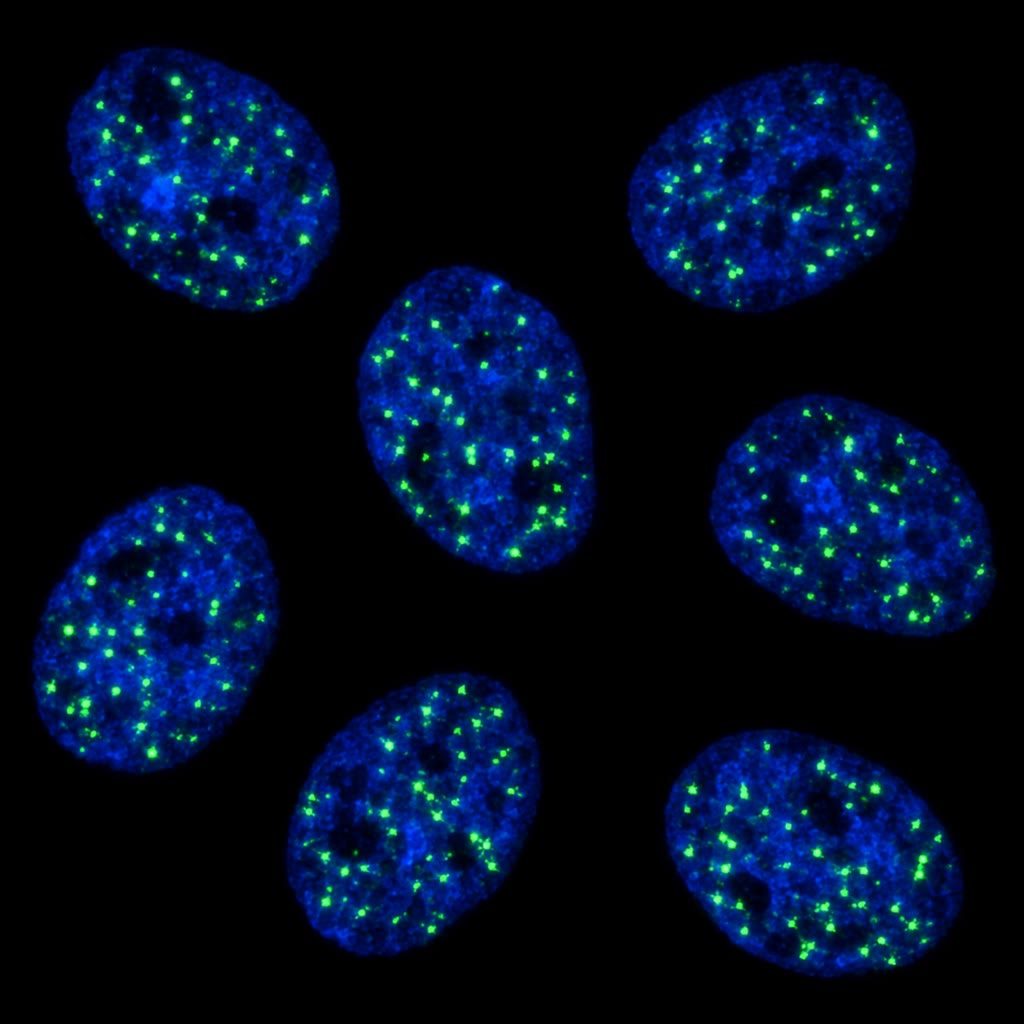
\includegraphics[width=0.4\linewidth]{images/book5/ai/b5-03-gamma-foci.jpg}

{\small विकिरण के एक घंटे बाद केंद्रकों (नीले) में $\gamma$-H2AX केंद्र
(हरे)। हर केंद्र किसी \omterm{def:b3:dna-repair:lesions}{द्विलड़ी विखंडन} को चिह्नित करता है; उन्हें गिनने
से क्षति और, अगले घंटों में, उसकी मरम्मत मापी जाती है।}
\end{omfigure}

\begin{example}[संश्लेषी घातकता: BRCA और PARP]\label{ex:b3:dna-repair:parp}
जिन स्त्रियों को \emph{BRCA1} या \emph{BRCA2} की एक दोषपूर्ण प्रति
वंशागत मिलती है उनमें स्तन-कर्कट का जीवन-काल जोखिम
\qtyrange{50}{80}{\%} होता है; अर्बुद उन्हीं कोशिकाओं में उठते हैं
जिन्होंने दूसरी प्रति भी खो दी है और जो अब \omterm{def:b3:dna-repair:dsb}{समजात पुनर्संयोजन} नहीं कर
सकतीं। ऐसी कोशिकाएँ अपने \omterm{def:b3:dna-repair:lesions}{द्विलड़ी विखंडनों} की मरम्मत केवल सिरा-संयोजन
से करती हैं और पुनर्विन्यास जमा करती हैं। वे एक विशिष्ट दुर्बलता भी पा
लेती हैं। एकलड़ी विखंडनों की, जो प्रति दिन कोई \num{10000} होते हैं,
मरम्मत ऐसे मार्ग से होती है जिसे एंज़ाइम PARP चाहिए; जब किसी औषध से
PARP निरुद्ध हो, तो एकलड़ी विखंडन S प्रावस्था तक बने रहते हैं, जहाँ कोई
द्विशाख हर एक को केवल एक सिरे वाले \omterm{def:b3:dna-repair:lesions}{द्विलड़ी विखंडन} में बदल देता है ---
जिसकी मरम्मत केवल पुनर्संयोजन से हो सकती है। किसी सामान्य कोशिका के
पास, जिसमें एक अच्छा \emph{\omterm{def:b3:dna-repair:dsb}{BRCA}} युग्मविकल्पी है, उपाय है; अर्बुद
कोशिका मर जाती है। दो दोष, जिनमें से हर एक अकेला हानिरहित है, साथ
मिलकर घातक हैं: औषध \emph{संश्लेषी घातकता} से मारती है और रोगी की
दूसरी कोशिकाओं को छोड़ देती है।
\end{example}

\begin{proposition}[औज़ार के रूप में पुनर्संयोजन]\label{prop:b3:dna-repair:tools}
\index{स्थल-विशिष्ट पुनर्संयोजन}\index{Cre-lox}
स्थल-विशिष्ट पुनर्संयोजक छोटे परिभाषित अनुक्रमों पर DNA को समजातता की
खोज या संश्लेषण के बिना काटते और फिर जोड़ते हैं: फ़ेज P1 का एंज़ाइम Cre
\qty{34}{bp} के \emph{loxP} स्थलों पर काम करता है, खमीर का एंज़ाइम Flp
\emph{FRT} स्थलों पर। एक ही अणु पर एक ही दिशा में दो स्थल उनके बीच का
DNA किसी वलय के रूप में उच्छेदित कर देते हैं; उलटी दिशाओं में वे उसे
प्रतिलोमित कर देते हैं; दो अणुओं पर पड़े स्थल अपने पार्श्व बदल लेते
हैं। \emph{loxP} स्थलों से घिरा (``फ़्लॉक्स्ड'') कोई जीन केवल उन्हीं
कोशिकाओं में विलोपित होता है जहाँ Cre अभिव्यक्त हो, प्रयोगकर्ता के चुने
किसी प्रवर्तक से, या प्रयोगकर्ता के चुने समय पर यदि Cre किसी औषध से
सक्रिय की जाए: भ्रूण के लिए अनिवार्य किसी जीन का अध्ययन वयस्क यकृत में,
या केवल किसी तंत्रिका-कोशिका में, इसी तरह होता है
(\cref{ch:b3:genetic-engineering})। कोशिका का अपना \omterm{def:b3:dna-repair:dsb}{समजात पुनर्संयोजन} ही
वह है जिसे जीन-लक्ष्यन और CRISPR-निर्देशित संपादन उधार लेकर कोई चुना
अनुक्रम किसी चुनी जगह लिखते हैं।
\end{proposition}

\begin{remark}[मरम्मत और वार्धक्य]\label{rem:b3:dna-repair:ageing}
जो कोशिकाएँ मरम्मत में विफल रहती हैं वे उत्परिवर्तन जमा करती हैं,
जराग्रस्त होती हैं या मर जाती हैं; मरम्मत के वंशागत दोष (वर्नर संलक्षण,
एक हेलिकेज़; कॉकेन संलक्षण, अनुलेखन-युग्मित मरम्मत; अनुमस्तिष्क-गतिभंग
केशिकाविस्फार, \omterm{def:b3:dna-repair:ddr}{ATM}) अकाल वार्धक्य के लक्षण पैदा करते हैं, और सामान्य
ऊतकों की कायिक उत्परिवर्तन-गणना आयु के साथ प्रति कोशिका प्रति वर्ष कोई
दसियों उत्परिवर्तन की दर से रैखिक रूप से बढ़ती है। जमा हुई क्षति
साधारण वार्धक्य का \emph{कारण} है या केवल उसके साथ चलती है, यह तय नहीं
है; यह बात अच्छी तरह समर्थित है कि मरम्मत की क्षमता जातियों के पार
जीवन-काल की एक निर्धारक है --- अधिक जीने वाली जातियाँ अधिक मरम्मत करती हैं।
\end{remark}

\section{अभ्यास}

\begin{exercise}[$\star$]\label{exo:b3:dna-repair:1}
इन \omterm{def:b3:dna-repair:lesions}{विक्षतियों} को स्वतःस्फूर्त या परिवेशी में वर्गीकृत कीजिए और हर एक के
लिए मरम्मत-पथ का नाम दीजिए: DNA में कोई यूरैसिल; कोई थाइमीन द्विलक; कोई
\omterm{def:b3:dna-repair:lesions}{8-ऑक्सोग्वानीन}; द्विशाख के पीछे कोई G--T असंगति; G1 में कोई \omterm{def:b3:dna-repair:lesions}{द्विलड़ी
विखंडन}।
\end{exercise}

\begin{exercise}[$\star$]\label{exo:b3:dna-repair:2}
\omterm{def:b3:dna-repair:excision}{न्यूक्लियोटाइड-उच्छेदन मरम्मत} को हर प्रकार की \omterm{def:b3:dna-repair:lesions}{विक्षति} के लिए विशिष्ट
एंज़ाइम की आवश्यकता क्यों नहीं, जबकि \omterm{def:b3:dna-repair:excision}{क्षार-उच्छेदन मरम्मत} को हर एक के
लिए एक \omterm{def:b3:dna-repair:excision}{ग्लाइकोसिलेज़} चाहिए?
\end{exercise}

\begin{exercise}[$\star$]\label{exo:b3:dna-repair:3}
\omterm{prop:b3:dna-repair:fidelity}{असंगति मरम्मत} की लड़ी-विभेदन समस्या बताइए और यह भी कि
\emph{E.~coli} उसे कैसे हल करता है। किसी \emph{dam} उत्परिवर्ती में
क्या होगा, जो किसी GATC स्थल का मेथिलीकरण नहीं करता?
\end{exercise}

\begin{exercise}[$\star$]\label{exo:b3:dna-repair:4}
किसी कोशिका को X-किरणों की \qty{2}{Gy} मात्रा मिलती है। मोटे तौर पर
उसमें कितने \omterm{def:b3:dna-repair:lesions}{द्विलड़ी विखंडन} होते हैं, और एक घंटे बाद आप कितने
$\gamma$-H2AX केंद्र गिनने की अपेक्षा करेंगे? छह घंटे बाद कम क्यों?
\end{exercise}

\begin{exercise}[$\star\star$]\label{exo:b3:dna-repair:5}
\cref{prop:b3:dna-repair:fidelity} का उपयोग करते हुए (क) किसी सामान्य
कोशिका, (ख) \omterm{prop:b3:dna-repair:fidelity}{असंगति मरम्मत} से वंचित किसी कोशिका, (ग) ऐसी कोशिका जिसकी
पॉलीमरेज़ अपना एक्सोन्यूक्लिएज़ खो चुकी है --- इनमें प्रति क्षार युग्म
उत्परिवर्तन-दर और प्रति द्विगुणित जीनोम प्रति विभाजन नए उत्परिवर्तनों
की संख्या निकालिए। कौन-सा अधिक खतरनाक उत्परिवर्तक है?
\end{exercise}

\begin{exercise}[$\star\star$]\label{exo:b3:dna-repair:6}
अक्षारीय स्थल प्रति कोशिका प्रति दिन $10^{4}$ की दर से उठते हैं और
\qty{15}{min} के अर्ध-आयु काल से मरम्मत होते हैं।
\cref{thm:b3:dna-repair:load} से किसी कोशिका में अक्षारीय स्थलों की
स्थायी-अवस्था संख्या निकालिए। यदि कोई औषध मरम्मत दस गुना धीमी कर दे तो
नई स्थायी अवस्था क्या है, और यदि कोई द्विशाख \qty{8}{h} में जीनोम की
नकल करे तो वह कितने स्थलों से मिलेगा?
\end{exercise}

\begin{exercise}[$\star\star$]\label{exo:b3:dna-repair:7}
G2 में किसी विखंडन की मरम्मत NHEJ (अर्ध-आयु \qty{30}{min}) या HR
(अर्ध-आयु \qty{4}{h}) से हो सकती है, दोनों उपलब्ध हैं। विखंडनों का
कितना अंश HR से जाता है? विखंडनों का अर्ध-आयु काल क्या है? फिर भी ढहे
प्रतिकृति द्विशाखों पर HR ही वह पथ क्यों है जो मायने रखता है?
\end{exercise}

\begin{exercise}[$\star\star$]\label{exo:b3:dna-repair:8}
(क) \omterm{def:b3:dna-repair:mmr}{लिंच संलक्षण}, (ख) \omterm{def:b3:dna-repair:excision}{ज़ीरोडर्मा पिग्मेंटोसम} समूह~A, (ग) Pol~$\eta$ से
वंचित XP-V विचरण वाले किसी रोगी के सूक्ष्म-उपग्रह व्यवहार, अर्बुद-वर्णक्रम
और धूप-संवेदनशीलता का पूर्वानुमान कीजिए।
\end{exercise}

\begin{exercise}[$\star\star$]\label{exo:b3:dna-repair:9}
किसी जीन के बहिर्वेशन~3 के दोनों ओर एक ही दिशा में दो \emph{loxP} स्थल
हैं; Cre ऐसे प्रवर्तक से अभिव्यक्त होता है जो जन्म से केवल यकृत में
सक्रिय है। वयस्क में यकृत-कोशिकाओं और तंत्रिका-कोशिकाओं का जीन-प्ररूप
बताइए, और यह भी कि यदि स्थल उलटी दिशाओं में रखे जाएँ तो क्या होगा।
\end{exercise}

\begin{exercise}[$\star\star\star$]\label{exo:b3:dna-repair:10}
LexA की प्रचालकों के प्रति आसक्तियों का उपयोग करते हुए समझाइए कि \omterm{prop:b3:dna-repair:sos}{SOS
अनुक्रिया} त्रुटि-प्रवण पॉलीमरेज़ों से पहले मरम्मत-जीन क्यों चालू करती
है, और यह भी कि जिस जीवाणु में त्रुटि-प्रवण पॉलीमरेज़ हों ही नहीं वह
प्रतिजैविकों से उपचारित किसी रोगी में फिर भी घाटे में क्यों हो सकता है।
\end{exercise}

\begin{exercise}[$\star\star\star$]\label{exo:b3:dna-repair:11}
कोई PARP निरोधक \emph{\omterm{def:b3:dna-repair:dsb}{BRCA}}-अपर्याप्त अर्बुद कोशिकाओं को मारता है पर
रोगी की सामान्य कोशिकाओं को नहीं। कारण-शृंखला बताइए, फिर उन दो तरीकों
का पूर्वानुमान कीजिए जिनसे कोई अर्बुद इस औषध के प्रति प्रतिरोधी बन सकता
है और आप हर एक को कैसे पकड़ेंगे।
\end{exercise}

\begin{exercise}[$\star\star\star$]\label{exo:b3:dna-repair:12}
किसी जीन-विनिमय पर जीन-परिवर्तन $3{:}1$ चतुष्क देता है। किसी चिह्नक पर
फैले विषमयुग्मक वाली कोई \omterm{def:b3:dna-repair:dsb}{हॉलिडे संधि} खींचिए (या उसका वर्णन कीजिए), और
दिखाइए कि विषमयुग्मक की \omterm{prop:b3:dna-repair:fidelity}{असंगति मरम्मत} एक दिशा में $3{:}1$ देती है,
दूसरी में $1{:}3$, और मरम्मत न हो तो ऐसा बीजाणु मिलता है जो स्वयं
विषमयुग्मजी है (अर्धसूत्रोत्तर पृथक्करण)। परिवर्तन जीन-विनिमय के पास के
चिह्नकों तक ही क्यों सीमित रहता है?
\end{exercise}

\section{समस्या: किसी जीनोम के जीवन का एक दिन}

\begin{problem}[{सप्तांत समस्या --- एक मानव कोशिका की दैनिक क्षति की
गणना, निष्ठा की सीढ़ी का गुणन, धूप की एक मात्रा का किसी सामान्य और किसी
मरम्मत-अपर्याप्त कोशिका में द्विशाख तक पीछा, X-किरणों की एक मात्रा का
दो मरम्मत-पथों में बँटवारा, और किसी अर्बुद की दुर्बलता का औषध में
बदलना, जिसका अंत द्विशाख से मिलते द्विलकों की संख्या, प्रति क्षार
उत्परिवर्तन-दर और पुनर्संयोजन से मरम्मत होने वाले विखंडनों के अंश पर
होता है}]
\label{pb:b3:dna-repair:1}
आँकड़े: किसी द्विगुणित मानव कोशिका में $6.4\times 10^{9}$ bp हैं, जिनमें
\qty{1.5}{\%} प्रोटीन-कूटलेखी हैं। प्रति दिन स्वतःस्फूर्त क्षति:
$10^{4}$ \omterm{def:b3:dna-repair:lesions}{विप्यूरीनन}, $400$ साइटोसीन \omterm{def:b3:dna-repair:lesions}{विअमीनन}, $10^{4}$ एकलड़ी
विखंडन। निष्ठा: पॉलीमरेज़ $10^{-5}$, शुद्धि-पाठन त्रुटियों का
$10^{-2}$ छोड़ता है, \omterm{prop:b3:dna-repair:fidelity}{असंगति मरम्मत} $10^{-3}$। एक धूप-स्नान प्रति
त्वचा-कोशिका $10^{5}$ \omterm{def:b3:dna-repair:lesions}{पिरिमिडीन द्विलक} छोड़ता है; उच्छेदन मरम्मत का
अर्ध-आयु काल सामान्यतः \qty{2}{h} और \omterm{def:b3:dna-repair:excision}{ज़ीरोडर्मा पिग्मेंटोसम} में
\qty{70}{h} है; कोई द्विशाख \qty{8}{h} बाद पहुँचता है; किसी द्विलक का
विक्षति-पार लाँघना प्रायिकता $10^{-3}$ से उत्परिवर्तन पैदा करता है।
X-किरणें प्रति ग्रे $35$ \omterm{def:b3:dna-repair:lesions}{द्विलड़ी विखंडन} बनाती हैं; NHEJ अर्ध-आयु
\qty{30}{min}, HR अर्ध-आयु \qty{4}{h}।

\medskip
\noindent\textbf{भाग I --- साधारण दिन।}
\begin{enumerate}
  \item कोशिका प्रति दिन और प्रति वर्ष कितनी स्वतःस्फूर्त \omterm{def:b3:dna-repair:lesions}{विक्षतियाँ}
        भोगती है? जीनोम के आकार से तुलना कीजिए।
  \item प्रति क्षार युग्म प्रति विभाजन उत्परिवर्तन-दर और प्रति विभाजन
        नए उत्परिवर्तनों की प्रत्याशित संख्या निकालिए।
  \item उनमें से कितने कूटलेखी अनुक्रम में पड़ते हैं? युग्मनज से किसी
        वयस्क त्वचा-कोशिका तक के मोटे तौर पर $50$ विभाजनों में कोई
        त्वचा-कोशिका केवल प्रतिकृति से कितने कूटलेखी उत्परिवर्तन ढोती
        है?
  \item \omterm{prop:b3:dna-repair:fidelity}{असंगति मरम्मत} से वंचित कोई कोशिका: उत्परिवर्तन-दर और प्रति
        विभाजन उत्परिवर्तन? \omterm{prop:b3:dna-repair:fidelity}{असंगति मरम्मत} के बिना कोई सूक्ष्म-उपग्रह
        $10^{4}$ विभाजनों में एक बार फिसलता है और उसके साथ $10^{7}$
        में एक बार। $10^{9}$ कोशिकाओं वाले ऐसे किसी अर्बुद में जो $40$
        विभाजनों से बना हो, हर स्थिति में कितनी कोशिकाएँ किसी दिए हुए
        सूक्ष्म-उपग्रह पर फिसला युग्मविकल्पी ढोती हैं? (दर $\times$
        विभाजन $\times$ कोशिकाएँ से आकलन कीजिए।)
  \item साइटोसीन का \omterm{def:b3:dna-repair:lesions}{विअमीनन} यूरैसिल देता है, 5-मेथिलसाइटोसीन का थाइमीन।
        किसकी मरम्मत होती है, किससे, और कौन उत्परिवर्तन बन जाता है?
        \cref{ch:b3:chromatin-epigenetics} की \omterm{def:b3:chromatin-epigenetics:methylation}{CpG} कमी से जोड़िए।
  \item कोई ऑक्सीकृत ग्वानीन (8-ऑक्सोG) प्रतिकृति के दौरान A से
        युग्मित होता है। कोशिका के पास C के सामने पड़े 8-ऑक्सोG के लिए
        एक \omterm{def:b3:dna-repair:excision}{ग्लाइकोसिलेज़} है, 8-ऑक्सोG के सामने पड़े A के लिए दूसरी, और
        ऐसी हाइड्रोलेज़ है जो ऑक्सीकृत dGTP को नष्ट कर देती है। बताइए
        कि हर एक क्या रोकती है और तीनों के विफल होने पर कौन-सा
        उत्परिवर्तन बनता है।
\end{enumerate}

\medskip
\noindent\textbf{भाग II --- धूप में एक दिन।}
\begin{enumerate}[resume]
  \item सामान्य और XP कोशिका के लिए उच्छेदन दर-नियतांक $k$ निकालिए।
  \item हर एक में द्विशाख पर कितने द्विलक बचे रहते हैं?
  \item हर स्थिति में धूप-स्नान प्रति कोशिका कितने उत्परिवर्तन पैदा
        करता है, और उनमें से कितने कूटलेखी अनुक्रम में हैं?
  \item ऐसे $500$ संपर्कों वाले बचपन में हर स्थिति में प्रति
        त्वचा-कोशिका कितने कूटलेखी उत्परिवर्तन? प्रश्न 3 की
        केवल-प्रतिकृति संख्या से तुलना कीजिए।
  \item लगभग $20$ जीन, जिनमें कुल \qty{40}{kb} कूटलेखी अनुक्रम है,
        उत्परिवर्तित होने पर किसी त्वचा-कर्कट को चला सकते हैं। XP
        बच्चे में प्रति कोशिका यह प्रायिकता क्या है कि धूप-प्रेरित
        कम-से-कम एक उत्परिवर्तन उनमें से किसी एक में पड़े? (सही माध्य
        के साथ पॉइसों का उपयोग कीजिए।) $10^{9}$ उद्भासित कोशिकाओं में
        कितनी पर चोट पड़ती है?
  \item समझाइए कि XP कोशिकाओं की समस्या द्विशाख की है, स्वयं \omterm{def:b3:dna-repair:lesions}{विक्षति}
        की नहीं, और कर्कट केवल त्वचा में ही क्यों प्रकट होते हैं।
\end{enumerate}

\medskip
\noindent\textbf{भाग III --- X-किरणों की एक मात्रा।}
\begin{enumerate}[resume]
  \item \qty{2}{Gy} की मात्रा: कितने \omterm{def:b3:dna-repair:lesions}{द्विलड़ी विखंडन}, और यदि NHEJ ही
        एकमात्र पथ हो (G1 कोशिका) तो एक घंटे बाद कितने
        $\gamma$-H2AX केंद्र?
  \item किसी G2 कोशिका में दोनों पथ चलते हैं। दर-नियतांक और HR से
        मरम्मत होने वाले विखंडनों का अंश निकालिए।
  \item G2 में विखंडनों का अर्ध-आयु काल क्या है, और एक घंटे बाद कितने
        बचते हैं?
  \item हर NHEJ घटना संधि पर कुछ क्षार युग्म बदल देती है। यदि कोई
        संधि प्रायिकता $0.015$ से कूटलेखी अनुक्रम में पड़े और तब वह
        बदलाव प्रायिकता $0.7$ से जीन को बिगाड़ दे, तो \qty{2}{Gy} की
        मात्रा प्रति G1 कोशिका कितने जीन बिगाड़ती है?
  \item $n$ युगपत् विखंडनों के साथ सिरे गलत जुड़कर कोई स्थानांतरण बना
        सकते हैं। मान लीजिए विखंडनों के $n(n-1)/2$ युग्मों में से हर
        एक प्रायिकता $3\times 10^{-4}$ से गलत जुड़ता है। \qty{2}{Gy}
        पर प्रति कोशिका प्रत्याशित स्थानांतरण? \qty{0.2}{Gy} पर? जोखिम
        मात्रा के वर्ग के साथ क्यों बढ़ता है जबकि विखंडनों की संख्या
        रैखिक रूप से बढ़ती है?
  \item वही \qty{2}{Gy} एक झटके के बजाय \qty{10}{h} में दी जाए: किसी
        एक समय पर कितने विखंडन उपस्थित रहते हैं (स्थायी अवस्था, NHEJ)?
        इसका स्थानांतरणों के लिए और विकिरण-चिकित्सा को खंडों में देने
        की प्रथा के लिए क्या अर्थ है?
  \item कोई कोशिका मात्रा $D$ से प्रायिकता $e^{-D/D_{0}}$ के साथ बचती
        है, जहाँ अक्षत मरम्मत वाली कोशिका के लिए
        $D_{0} = \qty{1.5}{Gy}$ और NHEJ से वंचित कोशिका के लिए
        \qty{0.5}{Gy} है। \qty{2}{Gy} और \qty{6}{Gy} पर हर एक की
        उत्तरजीविता निकालिए, और $D_{0}$ की व्याख्या कीजिए।
\end{enumerate}

\medskip
\noindent\textbf{भाग IV --- अर्बुद की दुर्बलता।}
\begin{enumerate}[resume]
  \item कोई \emph{BRCA2}-अपर्याप्त अर्बुद कोशिका विखंडनों की मरम्मत
        केवल NHEJ से करती है। प्रश्न 14 का उपयोग करते हुए बताइए कि
        उसके S/G2 विखंडनों का कितना अंश अब अयथार्थ ढंग से मरम्मत होता
        है जिसे कोई सामान्य कोशिका यथार्थ ढंग से करती। वर्षों में इससे
        उसके जीनोम का क्या होता है?
  \item PARP का निरोध प्रति दिन के $10^{4}$ एकलड़ी विखंडनों को
        बिना मरम्मत छोड़ देता है; उनमें से \qty{1}{\%} द्विशाखों से
        एक-सिरे वाले \omterm{def:b3:dna-repair:lesions}{द्विलड़ी विखंडनों} में बदल जाते हैं। प्रति कोशिका
        प्रति दिन ऐसे कितने विखंडन, और NHEJ किसी एक-सिरे वाले विखंडन
        की सही मरम्मत क्यों नहीं कर सकता?
  \item समझाइए कि \emph{BRCA2} के लिए विषमयुग्मजी रोगी की सामान्य
        कोशिकाएँ औषध से क्यों बच जाती हैं।
  \item कोई अर्बुद ऐसे दूसरे उत्परिवर्तन से प्रतिरोधी बन जाता है जो
        \emph{BRCA2} का वाचन-ढाँचा बहाल कर देता है। समझाइए, और बताइए
        कि आप उसे कैसे पकड़ेंगे।
  \item किसी क्षारकारी कारक से की गई रसायन-चिकित्सा अर्बुद कोशिकाओं को
        \omterm{prop:b3:dna-repair:fidelity}{असंगति मरम्मत} के ज़रिए मारती है: एंज़ाइम क्षारकृत क्षारों की
        मरम्मत का प्रयास करती है और कोशिका-मृत्यु चालू कर देती है।
        किसी लिंच-संलक्षण अर्बुद पर, जिसमें \omterm{prop:b3:dna-repair:fidelity}{असंगति मरम्मत} नहीं है,
        औषध के प्रभाव का पूर्वानुमान कीजिए।
  \item तीनों परिणाम बताइए: XP कोशिका में द्विशाख से मिलते द्विलक
        (प्रश्न~8), सामान्य प्रति क्षार युग्म उत्परिवर्तन-दर
        (प्रश्न~2), और G2 विखंडनों का वह अंश जिसकी मरम्मत HR करता है
        (प्रश्न~14)।
\end{enumerate}
\end{problem}
